\section{Network on Chip}

\nocite{HenessyPattersonCAQA}
\nocite{AC5}
\nocite{HenessyPattersonF}
\nocite{Duato03}
\nocite{YalamanchiliPCS}
\nocite{DeMicheli2006NetworksTools}

\subsection{Características de la red}
\begin{frame}{Características de la red I}
    \begin{minipage}[t]{.5\textwidth}
        \begin{figure}
            \centering
            \caption{Topología en malla indirecta}
            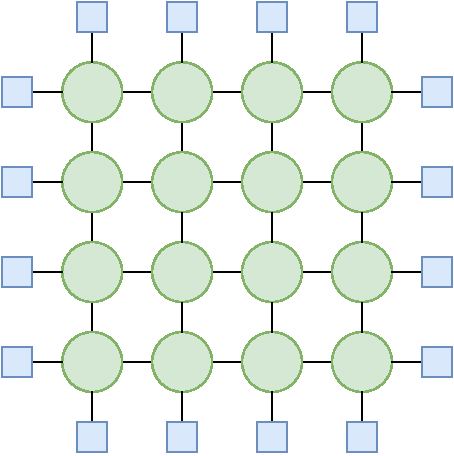
\includegraphics[width=.6\linewidth]{Images/topology_mesh_edge.drawio.pdf}
            \label{fig:topology}
        \end{figure}
    \end{minipage}\pause\begin{minipage}[t]{.5\textwidth}
        \begin{figure}
            \centering
            \caption{Encaminamiento en Orden Dimensional}
            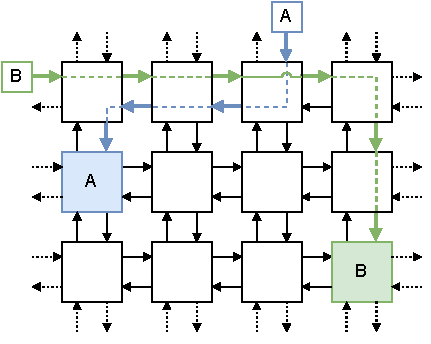
\includegraphics[width=.8\linewidth]{Images/dor2.drawio.pdf}
            \label{fig:routing}
        \end{figure}
    \end{minipage}
\end{frame}

\begin{frame}{Características de la red II}
    \begin{figure}
        \centering
        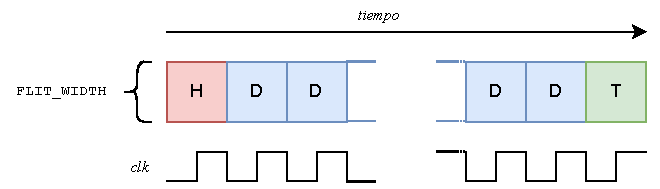
\includegraphics[width=.7\linewidth]{Images/packets.drawio.pdf}
        \caption{Envío de varios flits para formar un paquete.}
        \label{fig:packet}
    \end{figure}
\end{frame}

\subsection{Integración en el SweRV-EL2}

\begin{frame}{Modulos creados}
    \setbeamercovered{transparent}
    \begin{block}{Módulos de Red}
        \begin{itemize}[<+->]
            \item \textbf{Malla}: Instancia una malla bidimensional de \textit{router}s.
            \item \textbf{Router}: Hace de encaminador y tiene un \textit{crossbar}.
            \item \textbf{Crossbar}: Realiza la conmutación
        \end{itemize}
    \end{block}
    \onslide<+->
    \begin{block}{Módulos de Integración}
        \begin{itemize}[<+->]
            \item \textbf{Emisor}: Recibe un dato de longitud fija por un bus, lo empaqueta, y lo envía en una serie de flits por la red.
            \item \textbf{Receptor}: Recibe flits de la red, los desempaqueta en registros, y provee los resultados en un bus.
            \item \textbf{Wrapper}: Instancia un \textit{receptor}, el elemento de la EXU, y un \textit{emisor}.
        \end{itemize}
    \end{block}
\end{frame}

\begin{frame}{Integración de la NoC en el SweRV-EL2}
    \centering
    \only<1>{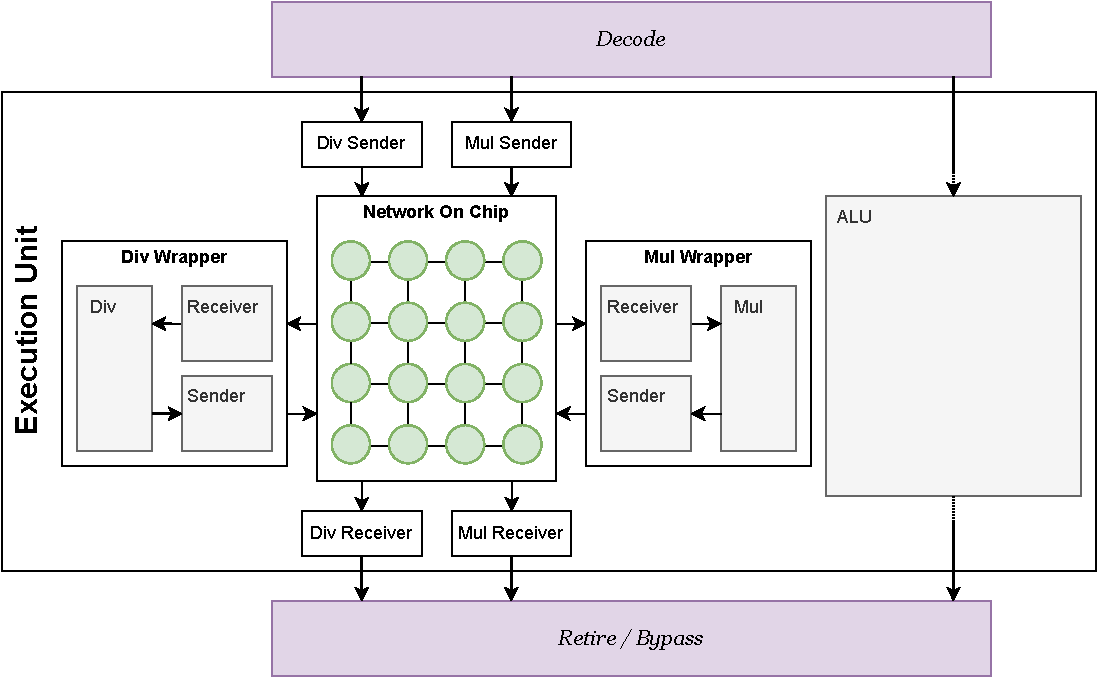
\includegraphics[height=.9\textheight]{Images/sketch_wrappers_horizontal.drawio.pdf}}
    \only<2>{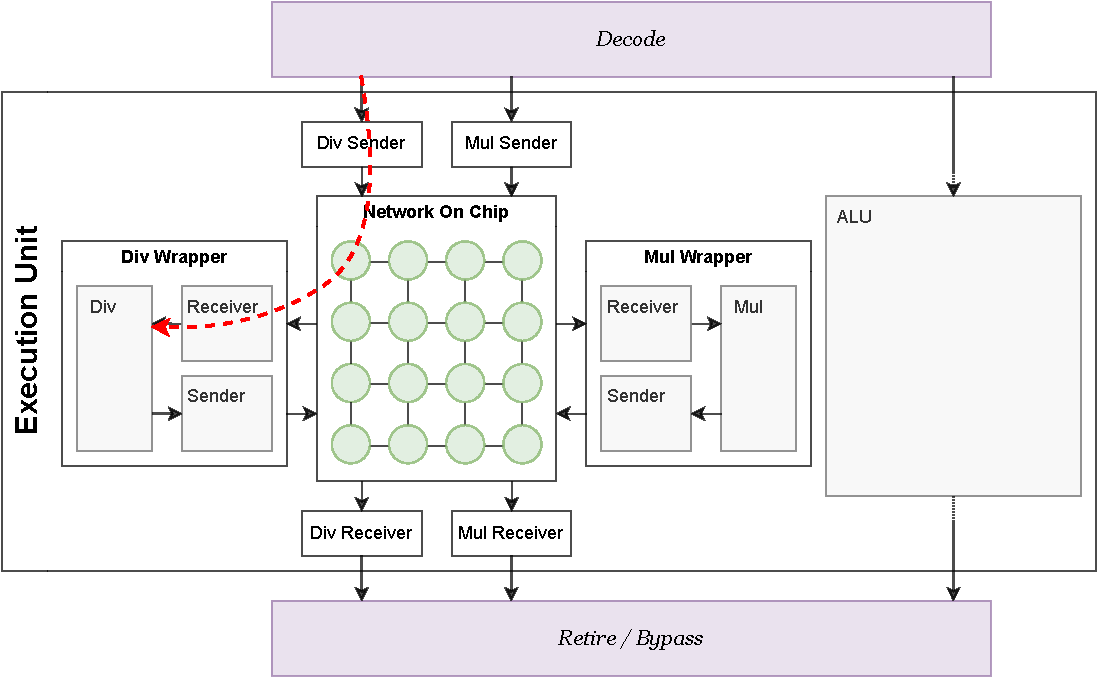
\includegraphics[height=.9\textheight]{Images/sketch_wrappers_horizontal-Page-3.drawio.pdf}}
    \only<3>{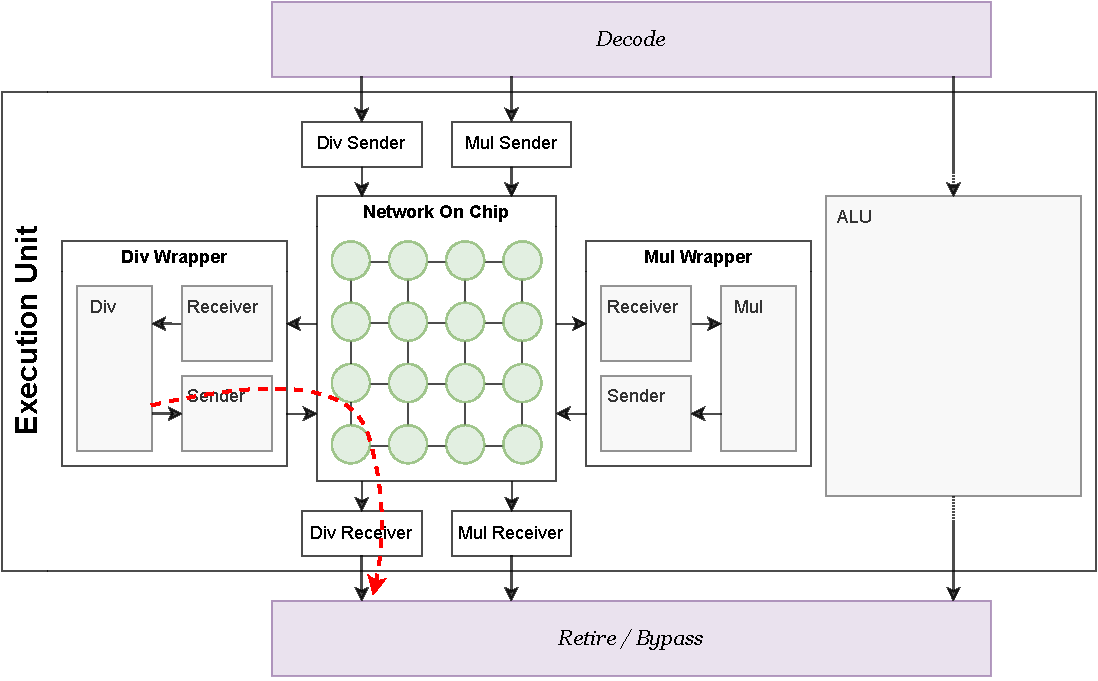
\includegraphics[height=.9\textheight]{Images/sketch_wrappers_horizontal-Page-4.drawio.pdf}}
\end{frame}